\documentclass[c]{beamer}

\usetheme{m}
\usepackage{FiraSans}
\usepackage[utf8]{inputenc}
\usepackage[british]{babel}
\usepackage{verbatim}
\usepackage{listings}
\usepackage{graphicx}

\title{Waking up with Perl 6}
\author{Paul Cochrane (\texttt{ptc})}

\begin{document}

\begin{frame}
    \titlepage{}
\end{frame}

\begin{frame}
    \begin{itemize}
        \item purely hypothetical talk
            \pause{}
        \item imagine you're at a conference
            \pause{}
        \item you haven't charged your smartphone for a long time
    \end{itemize}
    \centering{%
        
\includegraphics[width=0.6\textwidth]{battery-very-empty.jpeg}
    }
\end{frame}

\begin{frame}
    \begin{itemize}
        \item you plug it in\ldots
            \pause{}
        \item and it turns into this
    \end{itemize}
    \centering{%
        
\includegraphics[width=0.6\textwidth]{old-brick.jpeg}
    }
\end{frame}

\begin{frame}
    \begin{itemize}
        \item \ldots but it was your alarm clock!
    \end{itemize}
    \centering{%
        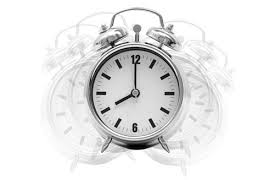
\includegraphics[width=0.6\textwidth]{alarm-clock-ringing.jpeg}
    }
\end{frame}

\begin{frame}[fragile]
    \begin{itemize}
        \item what do you do?
            \pause{}
        \item do you\ldots
            \begin{itemize}
                \item wake staff in hotel at 2.30am to ask for a wakeup call?
                    \pause{}
                \item install an alarm clock program on your laptop?
                    \pause{}
                \item use Perl 6?
            \end{itemize}
            \pause{}
        \item Perl 6 \texttt{sleep*} functions were documented Tuesday this week
        \item \url{http://doc.perl6.org/type/Temporal}
        \item \texttt{sleep-till(Instant \$till --> Bool)}
        \begin{itemize}
            \item which sleeps until the specified \texttt{Instant}
            \item if \texttt{Instant} is in the future, returns \texttt{True} when finished
            \item if \texttt{Instant} is in the past, returns \texttt{False} immediately
        \end{itemize}
    \end{itemize}
\end{frame}

\begin{frame}
    \begin{itemize}
        \item so\ldots
            \pause{}
        \item define the time for the alarm with \texttt{DateTime}
        \item convert that into an \texttt{Instant}
        \item be careful with timezones
            \begin{itemize}
                \item \texttt{DateTime.new} returns UTC by default
            \end{itemize}
        \item sleep until the relevant time
        \item wake up and start playing mp3s
    \end{itemize}
\end{frame}

\begin{frame}[fragile]
    \vfill
    \begin{verbatim}
    my $timezone = DateTime.now.timezone;
    my $instant = DateTime.new(
        year => 2015,
        month => 9,
        day => 4,
        hour => 7,
        minute => 0,
        timezone => $timezone
    ).Instant;
    sleep-till $instant;
    qqx{mplayer wake-me-up.mp3};
    \end{verbatim}
\end{frame}

\begin{frame}[fragile]
    \begin{itemize}
        \item it worked!
    \end{itemize}
    \huge
    \begin{verbatim}
            \o/
    \end{verbatim}
\end{frame}

\begin{frame}
    \begin{itemize}
        \item (yes, one could have used an \texttt{at} job)
        \item but where's the fun in that?
    \end{itemize}
\end{frame}

\begin{frame}
    % thanks to Larry for Perl
    \vfill
    \centering{%
        
\includegraphics[height=0.9\textheight]{larry-wall-wikipedia.jpeg}
    }
\end{frame}

\begin{frame}
    % thanks to Perl 6 hackers for Perl 6
    \centering{%
        \resizebox{!}{0.15\textheight}{\#perl6}
    }
\end{frame}

\begin{frame}
    % thanks to Split Enz for waking me up this morning
    \centering{%
        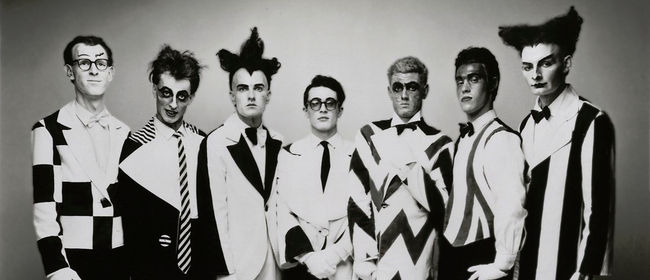
\includegraphics[width=0.9\textwidth]{split-enz.jpg}
    }
\end{frame}

\begin{frame}
    \centering{%
	\huge{Thanks!}
    }
\end{frame}

\end{document}

% vim: expandtab shiftwidth=4
